\documentclass[preprint,natbib]{sigplanconf}

\usepackage{amsmath}
\usepackage{../Utils}

\begin{document}

\conferenceinfo{Haskell Symposium '08}{September 25, 2008, Victoria, British Columbia, Canada.} 
\copyrightyear{2008} 
\copyrightdata{[to be supplied]} 

\titlebanner{Draft, to be submitted to Haskell Symposium '08}        % These are ignored unless
\preprintfooter{}   % 'preprint' option specified.

\title{Haskell as an Architecture Description Language}
%\subtitle{}

\authorinfo{Martijn M. Schrage \and S. Doaitse Swierstra}
           {Utrecht University}
           {\{martijn,doaitse\}@cs.uu.nl}

\maketitle

\begin{abstract}
We define a domain specific embedded language in Haskell for describing
layered software architectures which maintain bidirectional dependencies. By using a typed programming
language to describe the architecture, the type correctness of its components
is guaranteed by the type checker of the language. Because, contrary to the situation with typical Architecture Description Languages, the
description is part of the implementation of the
system, the implementation is guaranteed to comply with the architecture, and the architecture is guaranteed to comply with the implementation.
\end{abstract}

\category{D.2.11} {Software Engineering}
                  {Software Architectures}
                  [Languages (e.g., description, interconnection, definition)]

\terms
Domain-specific languages, Architecture

\keywords
Haskell, Layered architectures, Architecture descriptions, Type-level programming


\bc
f hor vert = (vert, hor) is most logical, but looks strange
f vert hor = (vert, hor) looks better but doesn't make it logical to parameterize f with its hor arg
f hor vert = (hor, vert) is chosen in thesis. result is a bit weird because vert is more logical on the left
\ec

\section{Introduction}\label{sect:introduction}

In this paper we develop a set of Haskell combinators for describing architectures of layered systems. Although designed with a layered editor in mind, we claim this approach to be applicable to many kinds of layered architectures. The combinators have been successfully used in the implementation of the generic editor Proxima~\cite{Schrage04Proxima}, as well as for a system providing web-interfaces to databases. 

Describing an architecture in an real programming language not only makes it possible to describe the interfaces of the components of the system, and how they are to be composed, but also enables us to smoothly extend this high-level description into a real implementation, without having to maintain several views on our system, with all its problems of diverging versions. Because the architecture description in Haskell is a program in itself, the system can be instantiated by providing implementations for each of the components.

In their survey of architecture description languages~\cite{medvidovic00ADLs}, Medvidovic and Taylor identify three essential components of an architecture description: a description of the (interface of the) components, a description of the connectors, and a description of the architectural configuration. They claim that the focus on {\em conceptual} architecture and explicit treatment of connectors as first-class entities differentiate architecture description languages from, amongst others, programming languages. However, Haskell offers possibilities for describing the main components of an architecture, while incorporating  these components as part of the program itself. Furthermore, by using abstraction, the description of the architecture can be focused on the conceptual architecture, while the details are left to the actual components.

As argued by Hudak~\cite{hudak98DSLs}, higher-order typed functional languages offer excellent possibilities for embedding domain-specific languages. Embedding a domain-specific language facilitates reuse of syntax, semantics, implementation code, software tools, as well as look-and-feel. In this paper we develop a DSEL in Haskell for describing layered editor architectures. We use records that contain functions to describe the components of the architecture. The connectors are combinators, and the configurations are programs (functions) that consist of combinators and components. 

In this paper we give three implementation models for layered architectures. First, in Section~\ref{sect:simpleEditor}, we introduce a simplified layered editor architecture and, in section~\ref{sect:layerInHaskell}, explore how its main components can be modeled in Haskell. Then we proceed to connect the components. In Section~\ref{sect:simple} the connection is straightforward, with little abstraction. This is used as a basis in Section~\ref{sect:ncp} as a base to develop a more abstract combinator implementation that uses nested pairs. In Section~\ref{sect:hidden}, we present another set of combinators, which employ a form of state hiding to improve on the previous set. Section~\ref{sect:lib} develops a small generic library for building the architecture-specific combinators of Section~\ref{sect:hidden}. The combinators from this section require two minimal function definitions for instantiating a specific architecture. In Section~\ref{sect:typeClass}, we exploit the type system to automatically provide these definitions, based solely on the types of the layer interface. Section~\ref{sect:proxima} shows how the architecture combinators are used to describe (and implement) the architecture of the Proxima editor. And, finally, Section~\ref{sect:conclusions} discusses future work and concludes.
			
			
			
\section{A simple editor}\label{sect:simpleEditor}

The architecture description combinators in this paper have been designed for the generic presentation-oriented structure editor Proxima. Proxima supports editing on the document structure as well as on its presentation, which has given rise to its layered architecture. A typical feature of the architecture is that each layer maintains its own local state, which is used to store information that does not have a logical place on the other layers. An example of this is white space, which is part of the presentation of a program source, but does not fit well in the abstract syntax tree. 

Because of the complexity of the actual Proxima architecture, we introduce a simple layered architecture for a presentation-oriented editor to explain the architecture description methods in the next sections. Although the architecture is simple, it contains the essential features of the Proxima architecture. 


Figure~\ref{simpleeditprocess} depicts the editing process for our simple editor. The editor keeps track of a document (\p{doc}), which is mapped onto a presentation (\p{pres}). The presentation process is split into $n$ steps: $\mathtt{present}_1 \dots \mathtt{present}_{n}$, each step takes care of a specific subtask, such as computing a set of layout alternatives, computing minimal and maximal sizes, negotiation between objects to be displayed about the available screen space, keeping track of white space which was explicitly entered by the user but which does not play a role at the document level and keeping track of explicit representation choices --toggling visibility, alignment, unfolding status-- made by the user in the course of the editing process. At the bottom of the figure, the presentation is shown to a user, who provides an edit gesture (\p{gest}) in response. The edit gesture is mapped onto a document update (\p{upd}) by $\mathtt{interpret}_{n} \dots \mathtt{interpret}_1$, which is then applied to the document. In the next cycle, the updated document is presented again. Note that some of the editing gestures effectively turn out to be identity operations at the top level, since some of them will be handled at an intermediate level, and will result in an update of the state maintained at that level.


A layer consists of a pair of $\mathtt{present}_i$ and $\mathtt{interpret}_i$ functions, which we refer to as {\em layer functions}. Besides the vertical data flow for presentation and interpretation, we thus may also have horizontal data flow that stays within the layer. Horizontal data flow is used to maintain state in a layer; this state component is passed along between all  computations taking place in a layer.


Figure~\ref{simplesinglelayer} shows the data flow for a single layer with two examples of horizontal data flow. The result \p{map} of the function \p{present} is passed on to \p{interpret} and represents information about where things are mapped on the screen. Furthermore, a \p{state} parameter is passed to \p{present} as well as \p{interpret}, and may be updated by \p{interpret}. Note that the \p{state} parameter of \p{present} is the result of \p{interpret} in the previous edit step. Because of the sequential nature of the edit steps, we only consider horizontal data flow that goes from left to right.





\begin{figure}
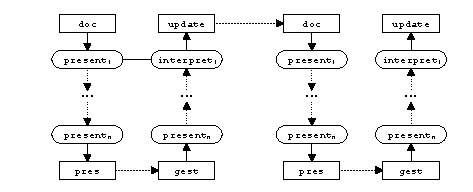
\includegraphics[width=\columnwidth]{images/EditCycles}
\caption{Two cycles in the editing process.}\label{simpleeditprocess} 
\end{figure}



\begin{figure}
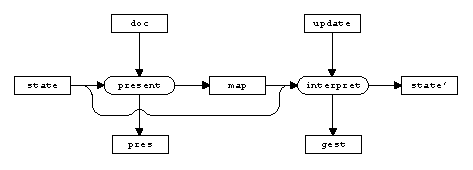
\includegraphics[width=\columnwidth]{images/SingleLayer}
\caption{A single layer.}\label{simplesinglelayer} 
\end{figure}





%																
%																
%																
\section{A layer in Haskell} \label{sect:layerInHaskell}

In the coming sections, we explore the possibilities of describing the layered architecture from the previous section in Haskell. There are two aspects to modeling a layered architecture in Haskell: the building blocks, which are the layer functions, and the connections between the building blocks. Before discussing how to model the connections between the layers, we focus of the functions within a layer.

A layer function takes  horizontal as well as vertical arguments and returns both  horizontal and vertical results. To make the difference between horizontal and vertical data explicit, we introduce a type synonym for layer functions.



%code Layers.hs
\begin{small}
\begin{verbatim}
type LayerFn horArgs vertArg horRess vertRes =
       horArgs -> vertArg -> (vertRes, horRess)
\end{verbatim}
\end{small}



Each layer is represented by a record containing all the layer functions: in our case \p{present} and \p{interpret}. The types of the layer functions follow directly from Figure~\ref{simplesinglelayer}.  If we  put these functions directly in a record, we  get:

%code Layers.hs
\begin{small}
\begin{verbatim}
data Simple state map doc pres gest upd =
       Simple { present   :: LayerFn state doc 
                                     map pres
              , interpret :: LayerFn (map,state) gest
                                     state upd
              }
\end{verbatim}
\end{small}


However, this is not entirely what we want. To simplify the horizontal connection between layer functions, we prefer a normalized data type in which the horizontal result type (\p{horRes}) of a layer function matches the horizontal argument type (\p{horArg}) of the next layer function. For our example, this implies that the horizontal result of \p{present} has the same type as the horizontal argument of \p{interpret} and vice versa (since the result of \p{interpret} is the argument of \p{present} in the next edit cycle). Figure~\ref{wrapped} shows the data flow for the layer functions in the normalized type \p{Simple}. Because the conversion to a normalized type is straightforward, we do not show it here. The definition of the normalized \p{Simple} is:

\begin{small}
\begin{verbatim}
data Simple state map doc pres gest upd =
       Simple { present   :: LayerFn state doc 
                                     (map, state) pres
              , interpret :: LayerFn (map, state) gest
                                     state upd
              }
\end{verbatim}
\end{small}

Although a \p{Simple} layer consists of two layer functions, the final combinator library presented in this paper abstracts over this number and can be used for layers with arbitrary numbers of layer functions.

\begin{figure}
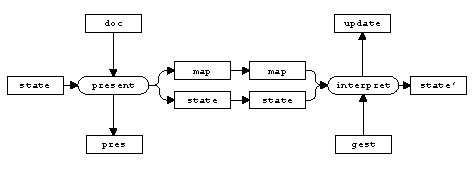
\includegraphics[width=\columnwidth]{images/NormalizedLayer}
\caption{Data flow in a normalized layer.}\label{wrapped} 
\end{figure}

			
\section{Method 1: Explicitly connecting the components} \label{sect:simple}

Now that the layers have been modeled, we need to realize the vertical data flow by connecting the layer functions. The document must be fed into the layers at the top, yielding the presentation at the bottom, and similarly, the edit gesture must be fed into the bottom layer, yielding the document update. The most straightforward way of tying everything together is to explicitly write down the selection and application of each of the functions in each of the layers. This will be the first approach, followed by gradually more abstract approaches in sections~\ref{sect:ncp} to \ref{sect:lib}.

We give an example edit loop that explicitly connects three layers: \p{layer1}, \p{layer2}, and \p{layer3} of type \p{Simple}. The data flow between the layer functions is shown in Figure~\ref{explicit}. Note that we might look at the code below as a textual representation of this picture, and that vice versa we might compute such a picture out of the code. At the bottom of the figure, the presentation is shown to the user, and an edit gesture is obtained, which we represent in the code with two functions \p{showRendering :: Rendering -> IO ()} and \p{getGesture :: IO Gesture}. At the top of the figure, the document is updated, which we model with a function \p{updateDocument :: Update -> Document -> IO Document}. The Haskell code for the edit loop is:


\begin{figure}
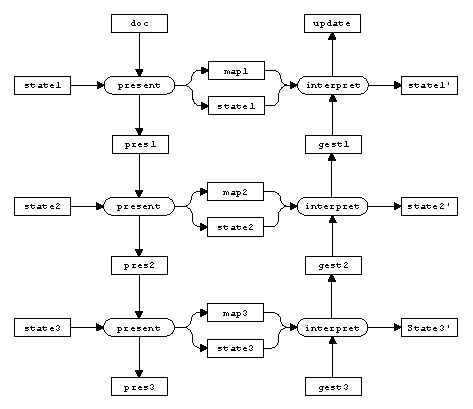
\includegraphics[width=\columnwidth]{images/LayersDataFlow}
\caption{Data flow in and between layers.} \label{explicit} 
\end{figure}

%code from Explicit.hs
\begin{small}
\begin{verbatim}
editLoop (layer1, layer2, layer3) states doc = 
  loop states doc where
  loop (state1, state2, state3) doc = 
   do { let (pres1,(map1,state1')) = 
              present layer1 state1 doc
      ; let (pres2,(map2,state2')) = 
              present layer2 state2 pres1
      ; let (pres3,(map3,state3')) = 
              present layer3 state3 pres2

      ; showRendering pres3
      ; gest3 <- getGesture

      ; let (gest2,state3'')  = 
              interpret layer3 (map3, state3') gest3
      ; let (gest1,state2'')  =
              interpret layer2 (map2, state2') gest2
      ; let (update,state1'') = 
              interpret layer1 (map1, state1') gest1
      
      ; let doc' = updateDocument update doc
      ; loop (state1'', state2'', state3'') doc'
      }
\end{verbatim}
\end{small}

The following function \p{main} calls \p{editLoop} with the correct parameters.
\newpage

%code from Explicit.hs
\begin{small}
\begin{verbatim}
main layer1 layer2 layer3 = 
 do { states <- initStates
    ; doc <- initDoc 
    ; editLoop (layer1, layer2, layer3) states doc
    }
\end{verbatim}
\end{small}

The functions \p{initStates} and \p{initDoc} provide the initial values for \p{states} and \p{doc}, and are left unspecified. The layers of the editor are arguments of the \p{main} function. An editor can now be instantiated by applying the function \p{main} to three \p{Simple} values each implementing a different layer. The type system verifies that the implemented layer functions have the correct type signatures.

A disadvantage of the implementation of the edit loop sketched in this section is that the patterns of the data flow are not very transparent. The fact that the state parameters are horizontal parameters and that the presentation is a vertical parameter is not immediately clear from the program code. Moreover, explicitly encoding the standard patterns for upward and downward vertical parameters, increases the chance of errors. Finally, the number of layers is hard coded in the implementation. If the system is extended with an extra layer, variables have to be renamed. If each type appearing in the layers is distinct, the type checker catches mistakes. However, type checking will not detect two equally typed variables accidentally being swapped. the goal of the coming sections is to gradually abstract from the current, very explicit description of the problem.


%																
%																
%																
\section{Method 2: Nested pairs}\label{sect:ncp}

\begin{figure}
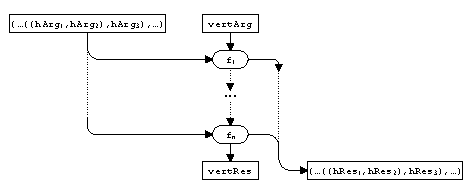
\includegraphics[width=\columnwidth]{images/NestedPairs}
\caption{Horizontal nested pairs for a downward step.}\label{ncp} 
\end{figure}


%\note{Ref to Doaitse Pablo?} 
In this section we abstract from the horizontal and vertical data-flow patterns in the edit loop of the previous section, by using combinators for combining layers. In the main loop, we call the layer functions of the combined layer, rather than explicitly calling each layer function in the main loop. The combinators also make the data flow more explicit. The direction of the vertical parameter is made apparent by the choice of combinator, rather than explicitly threading it through the function applications.

Similar to function composition ($f \cdot g$), we develop a \p{combine} combinator that takes two layers and returns a combined layer. The layer functions of the combined layer are compositions of the layer functions in the layers that are combined.

In the method described in this section, each of the functions in the combined layer not only takes a vertical argument and returns a vertical result, but it also takes a collection of horizontal arguments (one for each layer) and returns a collection of horizontal results (one from each layer). The \p{combine} combinator takes care of distributing the horizontal arguments to the corresponding layers, and also collects the horizontal results. The combined layer provides layer functions of type \p{LayerFn horArgC vertArg horResC vertRes}. The parameters \p{horArgC} and \p{horResC} stand for the types of the collections of horizontal parameters and results. Figure~\ref{ncp} sketches the data flow in the combined layer. Only one layer function with a downward vertical parameter is shown.

Because the types of the horizontal parameters are typically not of the same type, we cannot use a list to represent the collections. Moreover, we wish to be able to determine at compile time whether the collection contains the required number of elements. A tuple or cartesian product is more suitable for the task but has the disadvantage that its components cannot be accessed in a compositional way. Hence, we use a nested cartesian product to represent the horizontal parameters and results. 

We only use left-associatively nested products in this section: 
\p{(\dots((e$_1$,e$_2$),e$_3$), \dots ), e$_n$)}, although this will not be enforced by the combinators; as long as the structure of the argument and result products is the same, which is guaranteed by the way the \p{combine} combinator is used, the precise structure does not matter.


We first define two combinators for composing layer functions: a downward combinator \p{composeDown} (for \p{present}) and a upward combinator \p{composeUp} (for \p{interpret}). A downward vertical parameter passes through the higher layer first, whereas an upward vertical parameter passes through the lower layer first. Figure~\ref{composeDownUp} shows the data flow for the two combinators. 

The combinator \p{composeDown} composes two layers \p{higher} and \p{lower} by feeding the intermediate vertical result of \p{h} into \p{l}. At the same time, the horizontal parameters for \p{higher} and \p{lower} are taken from the horizontal parameter to the combined layer (which is a tuple), and the horizontal result for the combined layer is formed by tupling the horizontal results of \p{higher} and \p{lower}. 

%code from NCP.hs
\begin{small}
\begin{verbatim}
composeDown :: LayerFn horArgU arg horResU intr ->
               LayerFn horArgL intr horResL res ->
               LayerFn (horArgU, horArgL) arg 
                       (horResU, horResL) res
composeDown upper lower = 
  \(horArgU, horArgL) arg ->                                           
    let (interm, horResU) = upper horArgU arg
        (res, horResL)    = lower horArgL interm            
    in  (res, (horResU,horResL))
\end{verbatim}
\end{small}

\begin{figure}
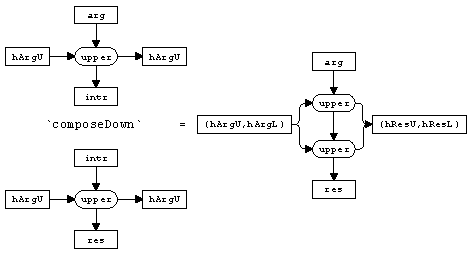
\includegraphics[width=\columnwidth]{images/ComposeDown}
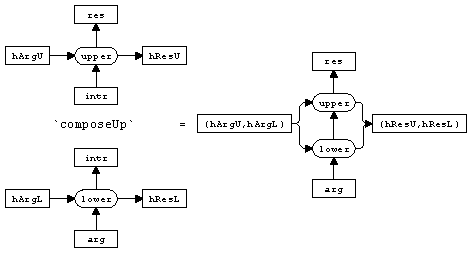
\includegraphics[width=\columnwidth]{images/ComposeUp}
\caption{\p{composeDown} and \p{composeUp}} \label{composeDownUp} 
\end{figure}


The definition of \p{composeUp} is analogous to \p{composeDown}. Its type is:

\begin{small}
\begin{verbatim}
composeUp :: LayerFn horArgU intr horResU res ->
             LayerFn horArgL arg horResL intr ->
             LayerFn (horArgU, horArgL) arg
                     (horResU, horResL) res
\end{verbatim}
\end{small}

\head{Combining layers}

Using \p{composeUp} and \p{composeDown}, we can now define a combinator to combine \p{Simple} layers. 


First, we need to define a new data type for combined layers. Although the composition of two layer functions is a layer function itself, we cannot use type \p{Simple} to represent a combined layer, because the types for the horizontal parameters do not match.  For \p{Simple}, the horizontal parameter of \p{present} has type \p{state}, and its result has type \p{(map, state)}. In contrast, the horizontal parameter of \p{present} in the composed layer is a nested pair of states and its result is a nested pair of \p{map} and \p{state} tuples. 

We introduce a type \p{LayerC} as a more general version of \p{Simple}. Because we cannot easily denote a nested pair structure in a Haskell type declaration, we leave the structure of the horizontal parameters unspecified. The parameter \p{states} represents the nested pair of \p{state} values, and the parameter \p{mapsStates} represents the nested pair of \p{map} and \p{state} tuples.

\begin{small}
\begin{verbatim}
data LayerC states mapsStates doc pres gest upd =
       LayerC { presentC ::   
                  LayerFn states doc mapsStates pres
              , interpretC :: 
                  LayerFn mapsStates gest states upd
              }
\end{verbatim}
\end{small}

The trivial function \p{lift} takes a layer of type \p{Simple} and returns a \p{LayerC} layer.

\begin{small}
\begin{verbatim}
lift :: Simple a b c d e f -> LayerC a (b,a) c d e f
lift simple = 
  LayerC { presentC = present simple
         , interpretC = interpret simple
         }
\end{verbatim}
\end{small}

The \p{combine} combinator is defined by using the appropriate \p{compose} combinator on each of the layer functions. 

\begin{small}
\begin{verbatim}
combine :: LayerC a b c d e f -> LayerC g h d i j e -> 
           LayerC (a,g) (b,h) c i j f
combine upper lower =
  LayerC { presentC = composeDown (presentC upper) 
                                  (presentC lower)
         , interpretC = composeUp (interpretC upper) 
                                  (interpretC lower)
         }
\end{verbatim}
\end{small}


\head{Simple editor}

The main editor loop from the previous section now reads:
 
\begin{small}
\begin{verbatim}
editLoop layers states doc = loop states doc
 where loop states doc = 
        do { let (pres, mapsStates) = 
                   presentC layers states doc
           
           ; showRendering pres
           ; gest <- getGesture
 
           ; let (update, states') = 
                   interpretC layers mapsStates gest
       
           ; let doc' = updateDocument update doc
           ; loop states' doc'
           }
\end{verbatim}
\end{small}

The \p{main} function is almost the same as in the previous section, except that instead of a 3-tuple of layers, the combined layers are passed to \p{editLoop}. 

\begin{small}
\begin{verbatim}
main layer1 layer2 layer3 = 
 do { (state1, state2, state3) <- initStates
    ; doc <- initDoc 
    ; let layers = lift layer1 `combine` lift layer2 
                               `combine` lift  layer3
    ; editLoop layers ((state1, state2), state3) doc
    }
\end{verbatim}
\end{small}

\head{Conclusions}

The nested pairs solution is more compositional than the approach of the previous section and most of the data flow is hidden from the main loop. However, the horizontal parameters are passed all the way through the composite layer, and are visible in the main loop, which is not where they conceptually belong. Moreover, the type of the composite layer is parameterized with all the types appearing in the layers, leading to large type signatures.




%																
%																
%																
\section{Method 3: Hidden parameters} \label{sect:hidden}

%Not fully abstracted factorized version of combinators primarily
%for explaining the model. Next section has more abstraction
%but is also harder to understand.
 
In the previous section, the horizontal results that are computed on evaluation of a combined layer function are returned explicitly and passed as arguments to the next layer function. In this section we take an alternative approach, which we explain with an example.  Recall that with the nested pairs method, each combined layer function returns a collection of horizontal results together with its vertical result:

\noindent
\dots\\
{\small \tt  let (pres, mapsStates) = presentC layers states doc }\\
\dots\\
{\small \tt let (update, states') = interpretC layers mapsStates gest}\\
\dots

In contrast, the hidden-parameter method does not return a collection of horizontal results, but a function that has already been partially applied to the horizontal results; the state is stored in the closure which is thus formed.

\noindent
\dots\\
{\small \tt let (pres, interpretStep) = presentStep doc}\\
\dots\\
{\small \tt let (update, presentStep') = interpretStep gest}\\
\dots

The code that is shown is not entirely accurate, but it gives the general idea. Together with the presentation, \p{presentStep} returns a function \p{interpretStep} for computing the document update. The layer functions in \p{interpretStep} have already been partially applied to the horizontal results from the presentation step. Thus, the horizontal parameters are now entirely hidden from the main loop, the main editor loop becomes more transparent and the type of a combined layer becomes simpler since the types for the horizontal parameters are internalized.


\head{Type definitions}

The type of the layer is described by the following type: 
\p{(Doc -> (Pres, Gest -> (Upd, Doc -> (Pres, Gest -> (Upd, \dots)))))}.  Unfortunately, we cannot use a type declaration: 

\begin{small}
\begin{verbatim}
type Layer = (Doc -> (Pres, Gest -> (Upd, Layer)))
\end{verbatim}
\end{small}


because Haskell does not allow recursive type synonyms. Hence, we need to use a \p{newtype} declaration, with the disadvantage that values of the type have to be wrapped with constructor functions.

\begin{small}
\begin{verbatim}
newtype Layer doc pres gest upd = 
          Layer ( doc -> 
                   ( pres, 
                       ( gest -> 
                           ( upd 
                           , Layer doc pres gest upd))))
\end{verbatim}
\end{small}

We now define two combinators for constructing and combining \p{Layer} values: \p{lift} converts  a \p{Simple} layer to a hidden-parameter layer of type \p{Layer}, and \p{combine} combines two layers of type \p{Layer}. Both combinators in this section are specific to the \p{Simple} type. In the next section, we define a library to construct \p{lift} and \p{combine} for arbitrary layers.


\head{Definition of \p{lift}}

The combinator \p{lift} takes a \p{Simple} layer and returns a \p{Layer}:

\begin{small}
\begin{verbatim}
lift :: Simple state map doc pres gest upd ->
        state -> Layer doc pres gest upd
lift simple state = presStep state 
 where presStep state = Layer $
         \doc ->  let (pres, (map,state)) = 
                        present simple state doc                                         
                  in  (pres, intrStep (map,state))
       intrStep (map,state) =
         \gest -> let (upd, state') = 
                        interpret simple (map,state) gest                     
                  in  (upd, presStep state')
\end{verbatim}%$
\end{small}
%\marginpar{state -> init omgedoopt}

Besides \p{layer}, \p{lift} gets a second parameter, \p{init}, which is the initial value of the horizontal parameter. The data flow pattern of the horizontal parameters is encoded entirely in the definition of \p{lift}. Moreover, the \p{state} type is not visible in the result of \p{lift}. Thus, once the initial horizontal state is passed to the lifted layer, it is no longer visible outside this layer; the \p{lift} combinator takes care of passing around the horizontal parameters between the layer functions, and also to the next edit cycle. 


\head{Definition of \p{combine}}

To combine layers, we define a combinator \p{combine}, which gets two layers as arguments: a higher layer and a lower layer. The type of \p{combine} is:

\begin{small}
\begin{verbatim}
combine :: Layer high med emed ehigh -> 
           Layer med low elow emed -> 
           Layer high low elow ehigh
\end{verbatim}
\end{small}

The reason for the order of the type variables is that for each pair of variables, the first type is an argument type and the second type  a result type. Hence, the first step in the combined layer is a function \p{high -> low}, which is the composition of a function \p{high -> med} in the higher layer and a function \p{med -> low} in the lower. On the other hand, the second step goes upward.  Thus, the function \p{elow -> ehigh} in the combined layer is the reverse composition of functions \p{elow -> emed} and \p{emed -> ehigh} in the higher and lower layers
  
The implementation of combine is just plumbing to get the parameters at the right places. The direction of the vertical parameters is encoded in the definition of \p{combine}. 


\begin{small}
\begin{verbatim}
combine = presStep
 where presStep (Layer upr) (Layer lwr) = Layer $ 
           \high -> let (med, uprIntr) = upr high
                        (low, lwrIntr) = lwr med
                    in  (low, intrStep uprIntr lwrIntr)
       intrStep upr lwr = 
           \elow -> let (emed, lwrPres) = lwr elow
                        (ehigh, uprPres) = upr emed
                    in  (ehigh, presStep uprPres lwrPres)
\end{verbatim}%$
\end{small}


\head{Simple editor}

The edit loop of the simple editor no longer contains references to the horizontal parameters. Furthermore, the combined layer is called \p{presentStep} instead of \p{layers} to reflect that it represents the presentation step of the computation.

\begin{small}
\begin{verbatim}
editLoop (Layer presentStep) doc = 
 do { let (pres , interpretStep) = presentStep doc
    
    ; showRendering pres
    ; gesture <- getGesture
    
    ; let (update, presentStep') = interpretStep gesture
    
    ; let doc' = updateDocument update doc
    
    ; editLoop presentStep' doc'
    }
\end{verbatim}
\end{small}

In the \p{main} function, the combined layer is created by lifting the layers together with their initial states and using \p{combine} to put them together.

\begin{small}
\begin{verbatim}
main layer1 layer2 layer3) =
 do { (init1, init2, init3) <- initStates
    ; doc <- initDoc 
    ; let layers = lift layer1 init1 `combine` 
                   lift layer2 init2 `combine`
                   lift layer3 init3
    ; editLoop layers doc
    }
\end{verbatim}
\end{small}

\head{Conclusions}

The hidden-parameter model hides the data flow of the horizontal parameters from the main loop of the system. Furthermore, the types of the horizontal parameters, as well as the intermediate vertical parameters, are hidden from the type of the composed layer. Thus, both horizontal and vertical data flow are made more transparent. 

%\note{monads arrows?} \note{relation to existential types. arrows?} 


%																
%																
%																
\section{Developing a library for architecture descriptions} \label{sect:lib}

In this section, we develop a small library for constructing \p{lift} and \p{combine} combinators for layered architectures having an arbitrary number of layer functions. We refer to these combinators as {\em meta combinators} because they are used to construct combinators.

The \p{lift} and \p{combine} combinators from the previous section are just one case of a layered architecture: a layer with two layer functions and hence two {\em step}s. Even though the combinators are straightforward, some code is duplicated, and small errors are easily made. Therefore, instead of a guideline on how to write \p{lift} and \p{combine} by hand, we prefer a small library of meta combinators for constructing these combinators. A further  advantage of having  a meta-combinator library is that instead of explicitly encoding the direction for each of the steps in the \p{combine} function, we can use the name of the meta combinator to reflect the direction in which the data flows (like with the \text{composeUp$/$Down} functions from the nested pairs method in Section~\ref{sect:ncp}).

Looking at the definitions of \p{lift} and \p{combine} in the previous section, we see that they both consist of two parts: one for each step in the layer. Both functions define a local function for each of the layer functions in the layer. In both \p{lift} and \p{combine} for the \p{Simple} layer type, these local functions are called \p{presStep} and \p{intrStep}. 

We derive the meta combinators by starting with the combinators from the previous section and gradually factoring out all step-specific aspects. We end with a combinator that is constructed out of a collection of simple building blocks (or meta combinators). 



 
%																
\subsection{Type definitions} \label{subsecttypedef}

\bc
oude todo{voor de eerste zin stond weer een kriebellijntje; ja, het type Layer heeft maar een constructor, en hier meb je het over "its constructors"; ik heb je oude paragraaf uitgecommentarieerd. Volgens mij bedoel je iets als:}



In the \p{Layer} type introduced in the previous section, the fact that we are dealing with two steps is explicitly encoded in the type. When dealing with more step-functions in a layer this type will get even more complicated. Since we do not want to ask from the user of the library to write  down such types explicitly, we start out by looking for a way of constructing such complicated types out of types which describe just a single step-function.
\ec


The \p{Layer} type poses a problem if we want to construct a library for building \p{lift} and \p{combine} functions, since somehow its constructors need to be added to and removed by the combinators. One solution is to create a type class for the constructor and deconstructor functions, but this complicates the types and requires a user to provide an instance of this class. Therefore, we introduce a compositional representation of a layer type that makes use of simple types defined in the library.

If we inspect the \p{Layer} type from the Section~\ref{sect:hidden}, we see it is made up of two steps of the form \p{vArg -> (vRes, ...)}. We  capture this in the following type:

\begin{small}
\begin{verbatim}
newtype Step a b ns = Step (a -> (b, ns))
\end{verbatim}
\end{small}

\bc
Using GADT's one might even make the fact that a step function should be seen as function by using the following formulation:

\begin{small}
\begin{verbatim}
newtype Step :: * -> * -> * where
  Step :: (a -> (b, ns)) -> Step (a -> b) ns
\end{verbatim}
\end{small}
\ec

In order to compose steps, we define an infix, right-associative, type constructor \p{(:.:)}.
The reason for right associativity will become apparent in Section~\ref{subsect:liftDerivation}.

\begin{small}
\begin{verbatim}
infixr :.:
newtype (:.:) f g ns  = Comp (f (g ns))
\end{verbatim}
\end{small}

We also define a \p{NilStep} as the starting point for a series of compositions:

\begin{small}
\begin{verbatim}
newtype NilStep t = NilStep t
\end{verbatim}
\end{small}

Now, for example, we can encode the type \p{Doc -> (Pres, Gest -> (Upd, next))} as
\p{(Step Doc Pres :.: Step Gest Upd :.: NilStep) next}. To encode the feedback loop, we introduce a fixed-point type \p{Fix}:

\begin{small}
\begin{verbatim}
newtype Fix f = Fix (f (Fix f))
\end{verbatim}
\end{small}

With these type combinators, we can now express \p{Layer} in a compositional and point-free way:

\begin{small}
\begin{verbatim}
type Layer doc pers gest upd = 
  Fix (Step doc pres :.: Step gest upd :.: NilStep)
\end{verbatim}
\end{small}

Because \p{Step}, \p{NilStep}, and \p{:.:}  appear partially parameterized in the layer type, and \p{Fix} is recursive, all three types need to be introduced using \p{newtype} definitions. Hence, instead of having a single \p{Layer} constructor, \p{lift} and \p{combine} will be littered with constructors. This is not a problem, however, since the combinators we will derive in the next subsections take care of adding and removing these constructors.

The reason why we have an explicit \p{NilStep} with yet another constructor is that it causes the number of occurrences (\p{:.:}) to be the same as the number of steps, which will facilitate the removal of \p{Comp} constructors. Furthermore, as we will see in Section~\ref{sect:typeClass}, the \p{NilStep} will also provide a base for recursive instances, preventing overlapping instances.


%																
\subsection{Derivation for \p{lift}}\label{subsect:liftDerivation}

First we develop a meta combinator for the \p{lift} function. We start with the code for \p{lift} for a layer with two steps from Section~\ref{sect:hidden}. If we rename several variables and adapt the code for the new constructor-rich representation of the \p{Layer} type, we get:


% from Derivation.hs (remove numbers of lift and combine in source file)
\begin{small} %lift0
\begin{verbatim}
lift simple state = step1 state 
 where step1 hArg = Fix . Comp . Step $
         \vArg -> let (pres, hRes) = 
                       present simple hArg vArg
                  in  (pres, step2 hRes)
       step2 hArg = Comp . Step $
         \vArg -> let (upd, hRes) = 
                        interpret simple hArg vArg
                  in  (upd, lNilStep hRes)
       lNilStep hRes = NilStep $ step1 hRes
\end{verbatim}%$
\end{small}

The definitions of the local functions \p{step1} and \p{step2} contain mutually-recursive references, thus hard-coding their position in the sequence of steps. We eliminate this positional information in the definitions by supplying the next step as a parameter to each function. The \p{lNilStep} no longer needs to be a local function.

%first drop state
%param now step1 gets step2 as param. but step2 has step1. instead of infinite
%definition lift layer = step1 (step2 (step1 ...., we make the observation that
%lift layer is step1 with the correct parameters, and hence pass lift layer as
%the parameter to step2, yielding the following finite definition:</comment></p> 
%\note{Johan: (over \p{lift layer} hieronder) "hier introduceer je een fixed point. Misschien iet meer woorden aan besteden?"} 
% ref: Augustson ICFP??
      
      
\begin{small} % lift1
\begin{verbatim}
lift :: Simple state map doc pres gest upd -> 
        state -> Layer doc pres gest upd
lift simple state =  
  step1 (step2 (lNilStep (lift simple))) state
 where step1 next hArg = Fix . Comp . Step $
         \vArg -> let (pres, hRes) = 
                        present simple hArg vArg
                  in  (pres, next hRes)
       step2 next hArg = Comp . Step $
         \vArg -> let (upd, hRes) = 
                        interpret simple hArg vArg
                  in  (upd, next  hRes)

lNilStep next hRes = NilStep $ next hRes
\end{verbatim}%$
\end{small}

Next we  capture the \p{Comp} and \p{Step} constructors and the lambda expression with the function \p{liftStep}. Here, it becomes apparent why composition is right associative, since each step has both a\p{Comp} constructor and a \p{Step} constructor. If composition were left-associative, the \p{Comp} constructors would end up between the \p{Fix} and \p{Step} constructors, and it would be harder to capture the pattern.

\begin{small} % lift2
\begin{verbatim}
liftStep f next horArgs = Comp . Step $ 
  \vArg -> let (vertRes, horRes) = f horArgs vArg
           in  (vertRes, next horRes)
\end{verbatim}%$
\end{small}

\noindent leading to the new definition of \p{lift}:

\begin{small} % lift2
\begin{verbatim}
lift simple state =
  step1 (step2 (lNilStep (lift simple))) state
 where step1 next hArg = 
         Fix $ liftStep (present simple) next hArg
       step2 next hArg =
         liftStep (interpret simple) next hArg 
\end{verbatim}%$
\end{small}



If we drop the \p{state} parameter on the first two lines and rewrite the function application as a composition, we get:
\
\begin{small}
\begin{verbatim}
lift layer = (step1 . step2 . lNilStep) (lift layer)
  ...
\end{verbatim}
\end{small}

\noindent Capturing the recursion pattern with the \p{fix} combinator:

\begin{small}
\begin{verbatim}
fix a = let fixa = a fixa
        in  fixa
\end{verbatim}
\end{small}

we get our next version of \p{lift}:

\begin{small} % lift4
\begin{verbatim}
lift simple = fix (step1 . step2 . lNilStep)
 where step1 next hArg = Fix $
         liftStep (present simple) next hArg
       step2 next hArg =
         liftStep (interpret simple) next hArg
\end{verbatim}
\end{small}%$


Regardless the number of steps, there will only be one \p{Fix} constructor (in contrast to the number of \p{Comp} and \p{Step} constructors, which are equal to the number of steps). Hence, we can define a function \p{lfix} to add this constructor. The function \p{lfix} also composes the \p{lNilStep} with the steps. 

\begin{small}% lift5
\begin{verbatim}
lfix f = fix f' where f' n = Fix . (f . lNilStep) n
\end{verbatim}
\end{small}


\begin{small}% lift5
\begin{verbatim}
lift simple = lfix (step1 . step2)
 where step1 next hArg = 
         liftStep (present simple) next hArg
       step2 next hArg = 
         liftStep (interpret simple) next hArg
\end{verbatim}
\end{small}

Now we got rid of the all the constructors in the local step definitions, we can drop the \p{next} and \p{args} parameters and give a point-free definition:

\begin{small} % lift
\begin{verbatim}
lift :: Simple state map doc pres gest upd ->
        state -> Layer doc pres gest upd
lift simple = lfix $ liftStep (present simple) 
                   . liftStep (interpret simple)
\end{verbatim}%$
\end{small}


\head{\p{liftStep} works for an arbitrary number of steps}

For an $n$-step layer, the definition of \p{lift} (using the method from Section~\ref{sect:hidden}) has $n$ local step functions, each  containing a reference to the next. \bc \note{mention that the last one refers to the first?} \ec For such a layer, we can perform exactly the same steps as for the 2-step \p{lift}. The resulting \p{lift} contains a composition of $n$ \p{liftStep} applications. If we denote the step type constructors by \p{Step$_i$} and the layer functions by \p{layerFn$_i$}, we get:

\begin{small}
\begin{tabbing}
{\tt lift layer = } \= {\tt lfix \$ liftStep (layerFn$_1$ layer)} \\
                    \>       \dots \\
                    \> {\tt .~~~~~~liftStep (layerFn$_n$ layer)}\\
\end{tabbing}%$
\end{small}

%Thus, we can use \p{liftStep} to define the \p{lift} combinator for a layer with any number of layer functions.


%																
\subsection{Derivation for \p{combine}} \label{subsubsectcombine}


The derivation of the meta combinators for \p{combine} is largely similar to the derivation for \p{lift}. We again start with the original definition of \p{combine} for a two-step layer, adapt it to the new \p{Layer} type and rename several variables:

\begin{small} % combine0
\begin{verbatim}
combine upr lwr = step1 upr lwr
 where step1 (Fix (Comp (Step upr))) 
             (Fix (Comp (Step lwr))) = 
         Fix . Comp . Step $ 
         \high -> let (med, uprIntr) = upr high
                      (low, lwrIntr) = lwr med
                  in  (low, step2 uprIntr lwrIntr)
       step2 (Comp (Step upr)) (Comp (Step lwr)) = 
         Comp . Step $
         \low -> let (med, lwrPres) = lwr low
                     (high, uprPres) = upr med
                 in  (high, cNilStep uprPres lwrPres)
       cNilStep (NilStep u) (NilStep l) = 
         NilStep $ step1 u l 
\end{verbatim}%$
\end{small}

The explicit mutual recursion in the local functions is removed by passing the next step as a parameter, and rewriting the whole function as a fixed point. The \p{cNilStep} becomes a top-level function.

\begin{small} %combine2
\begin{verbatim}
combine upr lwr = fix (step1 . step2 . cNilStep) upr lwr
 where step1 next (Fix (Comp (Step upr))) 
                  (Fix (Comp (Step lwr))) = 
         Fix . Comp . Step $ 
         \high -> let (med, uprIntr) = upr high
                      (low, lwrIntr) = lwr med
                  in  (low, next uprIntr lwrIntr)
       step2 next (Comp (Step upr)) (Comp ( Step lwr)) = 
         Comp . Step $
         \low -> let (med, lwrPres) = lwr low
                     (high, uprPres) = upr med
                 in  (high, next uprPres lwrPres)

cNilStep next (NilStep u) (NilStep l) = 
  NilStep $ next u l
\end{verbatim}%$
\end{small}

Without the explicit recursive calls, we can capture the vertical data flow patterns with two functions \p{combineStepDown} and \p{combineStepUp}:

\begin{small} 
\begin{verbatim}
combineStepDown :: (f x -> g y -> h ns) -> 
                   (Step a b :.: f) x -> 
                   (Step b c :.: g) y -> 
                   (Step a c :.: h) ns
combineStepDown next (Comp (Step upper)) 
                     (Comp (Step lower)) = Comp . Step $
  \h -> let (m ,upperf) = upper h
            (l, lowerf) = lower m
        in  (l, next upperf lowerf)   

combineStepUp :: (f x -> g y -> h ns) ->
                 (Step b c :.: f) x ->
                 (Step a b :.: g) y ->
                 (Step a c :.: h) ns
combineStepUp next (Comp (Step upper)) 
                   (Comp (Step lower)) = Comp . Step $ 
  \l -> let (m, lowerf) = lower l
            (h, upperf) = upper m
        in  (h, next upperf lowerf)   
\end{verbatim}%$
\end{small}

%Geldt ook combineStepUp next f g = combineStepDown (flip next) g f?
If we use these two functions, and drop the parameters to \p{step2}, we get:

\begin{small}%combine3
\begin{verbatim}
combine upr lwr = fix (step1 . step2 . cNilStep) upr lwr
 where step1 next (Fix upr) (Fix lwr) = 
         Fix $ combineStepDown next upr lwr
       step2 = combineStepUp
\end{verbatim}%$
\end{small}

The second step is now simply a \p{combineStepUp}, but the first step still contains a \p{Fix} constructor. In order to get rid of it, we first rewrite \p{combine} to make the pattern more apparent:

\begin{small}%combine4
\begin{verbatim}
combine = fix (\n (Fix u) (Fix l) -> 
  Fix $ (step1 . combineStepUp . cNilStep) n u l) 
 where step1 next upr lwr = 
         combineStepDown next upr lwr
\end{verbatim}
\end{small}%$

Now we can define a function \p{cfix} that pattern matches on the arguments and adds a \p{Fix} to the result. Similar to \p{lfix}, it also adds the \p{cNilStep}.

\begin{small}
\begin{verbatim}
cfix f = fix f' 
 where f' n (Fix u) (Fix l) = Fix $ (f . cNilStep) n u l
\end{verbatim}%$
\end{small}

which leaves us with:

\begin{small}% combine5
\begin{verbatim}
combine upr lwr = cfix (step1 . step2) upr lwr
 where step1 next upr lwr = 
         combineStepDown next upr lwr
       step2 = combineStepUp
\end{verbatim}
\end{small}


Now, we can drop the parameters and replace to \p{step1} and \p{step2} by \p{combineStepDown} and \p{combineStepDown}. Thus, the final version of \p{combine} reads

\begin{small}%combine
\begin{verbatim}
combine :: Layer high med emed ehigh ->
           Layer med low elow emed -> 
           Layer high low elow ehigh
combine = cfix (combineStepDown . combineStepUp)
\end{verbatim}
\end{small}


Similar to \p{liftStep}, \p{combineStepDown} and \p{combineStepUp} do not depend on the number of steps. Hence, they can be used to construct \p{combine} for layers with an arbitrary number of layer functions.


\head{Simple editor}

The \p{main} function for the simple editor is the same as in Section~\ref{sect:hidden}. Only the \p{editLoop} function has a couple of changes to account for the new constructors. To make the code more symmetric, we define deconstructor functions \p{unStep :: (Step a r :.: g) t -> a -> (r, (g t))} and \p{unNil} (which is the selector function of \p{NilStep}, when declared as a record.)

\begin{small}
\begin{verbatim}
unStep (Comp (Step step)) = step
unNil (NilStep step) = step

editLoop (Fix presentStep) doc = 
 do { let (pres , interpretStep) = 
            unStep presentStep $ doc
    
    ; showRendering pres
    ; gesture <- getGesture
    
    ; let (update, presentStep') =
            unStep interpretStep $ gesture
    
    ; let doc' = updateDocument update doc
    ; 
    ; editLoop (unNil presentStep') doc'
    }
\end{verbatim}%$
\end{small}



%																
\subsection{Adding a monad}


The final modification we make to the library is to add a monad, in order to allow layer functions to perform IO operations. The type \p{LayerFn} is extended with an extra type variable \p{m} for the monad.

\begin{small}
\begin{verbatim}
type LayerFn m horArgs vertArg horRess vertRes =
       horArgs -> vertArg -> m (vertRes, horRess)
\end{verbatim}
\end{small}

Consequentially, the \p{Step} type is also modified to account for the monadic result:

\begin{small}
\begin{verbatim}
newtype Step a b m ns = Step (a -> m (b, ns))
\end{verbatim}
\end{small}

At composition, the monad is passed to both arguments:

\begin{small}
\begin{verbatim}
newtype (:.:) f g m ns  = Comp (f m (g m ns))
\end{verbatim}
\end{small}

The \p{NilStep} does not actually use the monad argument:

\begin{small}
\begin{verbatim}
newtype NilStep m t = NilStep t
\end{verbatim}
\end{small}

For the fixed point, we introduce a type synonym \p{FixM}, which passes the monad to its type-function argument, and applies \p{Fix} to the result.

\begin{small}
\begin{verbatim}
type FixM m f = Fix (f m)
\end{verbatim}
\end{small}

The monadic version of the other code is largely similar to the non-monadic version. Basically, each let expression of the form\\

\noindent
\p{\small let x$_1$ = $exp_1$; \dots ; x$_n$ = $exp_n$ in ($hRes$,$vRes$)}\\

is replaced by a monadic statement\\

\noindent
\p{\small do \{ x$_1$ <- $exp_1$; \dots ; x$_n$ <- $exp_n$; return ($hRes$,$vRes$) \}}\\

Furthermore, the type signatures for the pairs of horizontal and vertical results \p{($hRes$, $vRes$)} become \p{m ($hRes$, $vRes$)}. Because of the similarity between the two libraries, we only show the monadic \p{liftStep}:

\begin{small}
\begin{verbatim}
liftStep :: (hArg -> vArg-> m (vRes, hRes)) -> 
            (hRes -> ns) -> hArg -> Step vArg vRes ns
liftStep f next horArgs = Step $ 
  \vArg -> do { (vertRes, horRes) <- f horArgs vArg
              ; return (vertRes, next horRes)
              }
\end{verbatim}
\end{small}%$

The functions \p{lfix}, \p{lcomp}, \p{cfix}, and \p{ccomp} are independent of the monad and are the same for both versions of the library.


%																
\subsection{Final Library and conclusions} \label{sect:libAndConclusions}

%from DPPMonad_Lib.hs
\begin{figure}
\begin{small}
\begin{center}
\begin{footnotesize}
\begin{verbatim}
fix :: (a->a) -> a
fix a = let fixa = a fixa
        in  fixa

type LayerFn m horArgs vertArg horRess vertRes =
       horArgs -> vertArg -> m (vertRes, horRess)


newtype FixM m f = Fix (f m)

infixr :.:

newtype (:.:) f g m ns  = Comp (f m (g m ns))

newtype NilStep m t = NilStep t

newtype Step a b m ns = Step (a -> m (b, ns))

unStep (Comp (Step step)) = step
unNil (NilStep step) = step


lfix f = fix f' where f' n = Fix . (f . lNilStep) n

lNilStep next hRes = NilStep $ next hRes

liftStep f next horArgs = Comp . Step $ 
  \vArg -> do { (vertRes, horRes) <- f horArgs vArg
              ; return (vertRes, next horRes)
              }
              

cfix f = fix f' 
 where f' n (Fix u) (Fix l) = Fix $ (f . cNilStep) n u l

cNilStep next (NilStep u) (NilStep l) = 
  NilStep $ next u l

combineStepDown next (Comp (Step upper)) 
                     (Comp (Step lower)) = Comp . Step $
  \h -> do { (m ,upperf) <- upper h
           ; (l, lowerf) <- lower m
           ; return (l, next upperf lowerf)   
           }

combineStepUp next (Comp (Step upper)) 
                   (Comp (Step lower)) = Comp . Step $
  \l -> do { (m, lowerf) <- lower l
           ; (h, upperf) <- upper m
           ; return (h, next upperf lowerf)
           }
\end{verbatim} %$
\end{footnotesize}\caption{Final meta-combinator library}\label{fig:metacombinators} 
\end{center}
\end{small}
\end{figure}

Figure~\ref{fig:metacombinators} contains the final monadic library. In order to describe and implement an architecture, we need to provide a \p{Layer} type, and definitions of \p{lift} and \p{combine}. We give a general description of these definitions.


\head{General use} 


The general case that we consider is a layer with $n$ layer functions. The record type \p{TheLayer m h$_1$ \dots ~h$_m$ a$_1$ r$_1$ a$_2$ r$_2$ \dots ~a$_n$ r$_n$} contains the layer functions. The variable \p{m} is the monad, variables \p{h$_i$} are the types that appear in the horizontal parameters of the layer, and the \p{a$_i$} and \p{r$_i$} are the types of the vertical arguments and results. 

Because the types of the horizontal parameters are not necessarily single \p{h$_i$} variables, but tuples of these variables, we denote the horizontal parameters by $horArgs_i$ and $horRess_i$. As an example, consider the type \p{Simple}. Its horizontal  type variables are \p{map} and \p{state}, but the types of the horizontal parameters are \p{state} and \p{(map, state)}. 

In general, the definition of \p{TheLayer} has this form:

\begin{small}
\begin{tabbing}
{\tt da}\={\tt ta}\\
\> {\tt Th}\={\tt eLayer~m h$_1$ \dots ~h$_m$ a$_1$ r$_1$ a$_2$ r$_2$ \dots ~a$_n$ r$_n$ = }\\
\> \> {\tt TheLayer~}\={\tt \{~LayerFn$_1$}\verb| :: |{\tt LayerFn~m~}\= {\tt $horArgs_1$ a$_1$}\\
\> \>                \>                                             \> {\tt $horArgs_2$ r$_1$}\\
\>\>\> {\tt , LayerFn$_2$}\verb| :: |{\tt LayerFn~m~}\={\tt $horArgs_2$ a$_2$}\\
\> \>                \>                            \>{\tt $horArgs_3$ r$_2$ \}}\\
\>\>\> {\tt \dots }\\
\>\>\> {\tt , LayerFn$_n$}\verb| :: |{\tt LayerFn~m~}\={\tt $horArgs_{n}$ a$_n$}\\
\> \>                \>                            \>{\tt $horArgs_1$ r$_n$ \}}\\
\end{tabbing}
\end{small}

We assume the layer is normalized, meaning that $horArgs_{1} = horRess_n$ and 
$horArgs_{i+1} = horRess_i$. If the layer is not normalized, a simple wrapper function can be defined to convert the layer to a normalized layer (see Section~\ref{sect:layerInHaskell}). 

\head{Type definitions}

For a layer record as defined above, the type definition for the \p{Layer} type used by the combinators is:

\begin{small}
\begin{tabbing}
{\tt ty}\={\tt pe Layer m a$_1$ r$_1$ a$_2$ r$_2$ \dots ~a$_n$ r$_n$ =}\\
        \>{\tt FixM m (Step a$_1$ r$_1$ :.: a$_2$ r$_2$ :.: \dots ~:.: Step a$_n$ r$_n$)}\\
\end{tabbing}
\end{small}


\head{Definition of \p{lift} and \p{combine}} 

The definitions of \p{lift} and \p{combine} are straightforward. For \p{lift}, we need to apply \p{liftStep} to each of the layer functions, compose the steps with \p{lcomp}, and apply \p{lfix} to the composition. 

\begin{small}
\begin{tabbing}
{\tt lift}\verb| :: |\={\tt Monad m =>}\\
                     \>{\tt TheLayer m h$_1$ \dots ~h$_m$ a$_1$ r$_1$ \dots ~a$_n$ r$_n$ ->}\\
                     \>{\tt Layer m a$_1$ r$_1$ \dots ~a$_n$ r$_n$}\\
{\tt li}\={\tt ft t}\={\tt heLayer = }\\
\>{\tt lfix \$ liftStep (LayerFn$_1$ theLayer)}\\
\>\verb|     . lift|{\tt Step (LayerFn$_2$ theLayer)}\\
\>{\tt ~~~~~\dots}\\ 
\>\verb|     . lift|{\tt Step (LayerFn$_n$ theLayer)}
\end{tabbing}
\end{small}%$


The \p{combine} combinator consists of $n$ \p{combineStepUp$/$Down} meta combinators, composed with \p{ccomp}, after which \p{cfix} is applied. The direction of the vertical data flow determines the choice between \p{combineStepUp} and \p{combineStepDown} for each step.  The exact type of \p{combine} depends on the direction of the meta combinators and is explained below. 

\begin{small}
\begin{tabbing}
{\tt combine}\verb| :: |\={\tt Monad m =>}\\
                        \>{\tt Layer m \dots}\verb| -> |{\tt Layer m \dots}\verb| -> |{\tt Layer m \dots }\\
{\tt co}\={\tt mbine}\={\tt ~= }\\
\>{\tt cfix \$ combineStepUp$/$Down}\\
\>{\tt ~~~~~\dots}\\ 
\>\verb|     . combine|{\tt StepUp$/$Down}\\
\end{tabbing}%$
\end{small}

The type of \p{combine} depends on the direction of the vertical data flow in the layer. Consider the $i$-th pair of  type variables in \p{Layer a$_1$ r$_1$ \dots~a$_n$ r$_n$}. Variable \p{a$_i$} represents the vertical argument of layer function $i$, and \p{r$_i$} the vertical result. If step $i$ is an upward step, the variables at this position in the \p{Layer} types are related as follows in the type signature for \p{combine}:

\begin{small}
\begin{tabbing}
{\tt  combine :: }\={\tt Monad m =>}\\
                  \>{\tt Layer \dots~md h \dots}\verb| -> |{\tt Layer \dots~l~md \dots} \verb| ->|\\
                  \>{\tt Layer \dots~l h \dots}\\
\end{tabbing}
\end{small}

On the other hand, for a downward layer function, we have:

\begin{small}
\begin{tabbing}
{\tt  combine :: }\={\tt Monad m =>}\\
                  \>{\tt Layer \dots~h md \dots}\verb| -> |{\tt Layer \dots~md l \dots} \verb| ->|\\
                  \>{\tt Layer \dots~h l \dots}
\end{tabbing}
\end{small}


\subsection{Conclusions} 

The meta combinator library has the advantages of the hidden-parameter solution from Section~\ref{sect:hidden}, but at the same time, it is much easier to describe a specific architecture. The use of meta combinators makes the data flow clearer and reduces the chance of errors in the specification. For a specific architecture, we only need to define a \p{Layer} type, and give simple definitions of \p{lift} and \p{combine}.









%																
%																
%																
\section{Type-class magic} \label{sect:typeClass}

The definitions of \p{lift} and \p{combine} that have to be provided manually for each specific architecture are almost uniquely determined by the layer type, which leads to the question whether we can use type classes to construct generic versions of these functions. Indeed, this turns out to be possible if we encode the direction of each step in its type. In this section, we present the type classes and instances that do the job. For clarity, we use the non-monadic combinators from Section~\ref{sect:lib} as a base.

To encode the direction of a step, we extend the \p{Step} type with a phantom-type variable~\cite{leijen99dsecs}.

\begin{small}
\begin{verbatim}
newtype Step dir a b ns = Step (a -> (b, ns))
\end{verbatim}
\end{small}

Two constructorless types encode the direction.

\begin{small}
\begin{verbatim}
data Up 
data Down 
\end{verbatim}
\end{small}



\head{Definition of \p{genericLift}}

A generic version of \p{lift} would take a variable number of layer functions, and returns a layer type . The number of layer functions is determined by the number of steps in the result type (which is determined by the context in which it is used.)

The structure of a generic version of \p{lift} in a pseudo-Haskell language would read:

\begin{small}
\begin{verbatim}
genericLift :: 
  lf1 -> .. -> lfn ->
  Fix (Step Up/Down <s1> :.: .. :.: Step Up/Down <sn>)
genericLift = \lf1 .. lfn -> 
              lfix (liftStep lf1 . ..  . liftStep lfn)
\end{verbatim}%$
\end{small}

In this code, we can identify a composition function that takes a varying number of functions (\p{liftStep lf1} to \p{liftStep lfn}) and return a composition. If we assume a function \p{compose}, that takes a representation of the number of steps (denoted by \p{<n>}) followed by \p{n} functions, we can rewrite \p{genericLift} to:

\begin{small}
\begin{verbatim}
genericLift = \lf1 .. lfn -> 
  lfix (compose <n> (liftStep lf1) .. (liftStep lfn))
\end{verbatim}%$
\end{small}

% this backslash somehow is not tt
Now, we can identify another pattern \p{ $\mathtt{\backslash}$a1 an -> f (g (h a1) .. (h an))}. Because of the parentheses around \p{g} and its arguments, we cannot simply compose \p{f} and \p{g}. We assume a function \p{app}, which takes the representation of the steps \p{<n>}, and the two functions \p{f} and \p{g}. For \p{h}, \p{app} uses \p{liftStep}, which is not a parameter. If we take \p{f} to be \p{lfix}, and \p{g} to be \p{compose <n>}, we have a new version of \p{genericLift}:

\begin{small}
\begin{verbatim}
genericLift = app <n> lfix (compose <n>)
\end{verbatim}%$
\end{small}

The final non-Haskell part in the definition is the \p{<n>} expression. The number of steps is represented by the argument of the \p{Fix} type in the result of \p{genericLift}. Hence, we assume a function \p{resType}, which for functions of type \p{a1 .. an -> Fix (s1 :.: .. :.: sn)} returns \p{steps t} (note that \p{steps} has kind \p{* -> *}). With this last function, the definition of \p{genericLift} is no longer pseudo code, but actual Haskell:

\begin{small}
\begin{verbatim}
genericLift = app (resType genericLift) lfix 
                  (compose (resType genericLift))
\end{verbatim}%$
\end{small}

Which leaves us the task of defining the type classes  for constructing the right instances for \p{compose}, \p{app}, and \p{resType}.

For the variable-argument composition \p{compose}, we declare a class \p{Comp} with a single method \p{comp}, which takes a composition type, and a neutral element, and returns a composition function that takes as many arguments as the composition type has steps. The function \p{compose} is simply \p{comp} with \p{id} for the neutral element.

\begin{small}
\begin{verbatim}
class Comp (cmp :: * -> *) r c | cmp -> r c where
  comp :: cmp t -> r -> c

instance Comp (NilStep) (b->res) (b->res)  where
  comp cmp r = r  

instance Comp g (a->res) cmp =>
         Comp (f :.: g) (y->res) ((a->y) -> cmp) where
  comp cmp r = \ab -> comp (rightType cmp) (r.ab)

rightType :: (f :.: g) t -> g t
rightType = undefined

compose c = comp c id
\end{verbatim}
\end{small}

The application function is a bit more complex. The class \p{App} has a method \p{app}, which takes a composition type, and two functions \p{f} and \p{fx}. The result is a function that has the same number of arguments as the composition type has steps, and which applies \p{fx} to each argument, and applies these arguments to the function \p{f}.

\begin{small}
\begin{verbatim}
class App (cmp :: * -> *) f fx r | cmp f -> fx r  where
  app :: cmp t -> f -> fx -> r

instance App (NilStep) (a->b) a b  where
  app cmp f a = f a

instance App g (a->b) d e =>
         App (Step dr ar rs :.: g) (a->b) 
              (((hRes -> g ns) -> hArg -> 
                (Step dr vArg vRes :.: g) ns) ->d) 
             (LayerFn hArg vArg hRes vRes ->e) where
  app cmp f fx = \lf -> (app (rightType cmp) f
                             (fx (liftStep lf))) 
\end{verbatim}
\end{small}

The code for \p{liftStep} is the same as in the previous section. Its type differs slightly due to the direction type variable, but since this is a phantom type, it does not show up in the values. 

The last problem we need to tackle is how to obtain the composition type over which \p{compose} and \p{app} recurse. For this we declare a class \p{ResType} with a method \p{resType}, which yields the result type of its function argument. Since the result of \p{genericLift} is always of type \p{Fix ct}, we can define a base instance for \p{Fix ct}, in which \p{restype} returns \p{ct t}, and a recursive instance for \p{a -> f}, in which \p{restype} returns the result type of \p{f}. Since no values are actually computed here, we can give the method a default implementation of \p{undefined}.


\begin{small}
\begin{verbatim}
class ResType f res | f -> res where
  resType :: f -> res
  resType = undefined

instance ResType (Fix ct) (ct t)
  
instance ResType f r => ResType (a -> f) r
\end{verbatim}
\end{small}



\head{Definition of \p{genericCombine}}

The situation for \p{genericCombine} is somewhat simpler than for \p{genericLift}, since the function does not have a varying number of arguments. However, unlike \p{genericLift}, the step functions are based on the direction of the step. If we look at \p{genericCombine}, the general structure would be:

\begin{small}
\begin{verbatim}
combine :: 
  Fix (Step Up/Down .. :.: .. :.: Step Up/Down .. ) ->
  Fix (Step Up/Down .. :.: .. :.: Step Up/Down .. ) ->
  Fix (Step Up/Down .. :.: .. :.: Step Up/Down .. )
combine = cfix \$ combineStepUp/Down 
                  ...
                . combineStepUp/Down 
\end{verbatim}%$
\end{small}

We assume a function that creates a composition of \p{n} combine steps, where the choice for an upward or a downward step is based on the direction of the respective \p{Step} type in the composition type.


\begin{small}
\begin{verbatim}
genericCombine = cfix (combineC (resType genericCombine))
\end{verbatim}%$
\end{small}

The type class looks a bit unfriendly due to the presence of the \p{Step} type, which is necessary because of the dependence on the direction.

\begin{small}
\begin{verbatim}
class Combine (cmp :: * -> *) t f | cmp t -> f where
  combineC :: cmp t -> f

instance Combine NilStep t ((x -> y -> t) -> 
          (NilStep x) -> (NilStep y) -> NilStep t) where
  combineC _ = \next (NilStep x) (NilStep y) ->
                 NilStep (next x y) 
 
instance (Combine c ct ( (ut -> lt -> ct) ->
                        u ut -> l lt-> c ct) ) =>
         Combine (Step Down a r :.: c) ct
                 ((ut -> lt -> ct) ->
                  (Step Down a m :.: u) ut -> 
                  (Step Down m r :.: l) lt -> 
                  (Step Down a r :.: c) ct) where
  combineC cmp = \next u l ->
    combineStepDown (combineC (rightType cmp) next) u l
\end{verbatim}
\end{small}

\bc
instance (Combine c ct ( (ut -> lt -> ct) ->
                        u ut -> l lt-> c ct) ) =>
         Combine (Step Up a r :.: c) ct
                 ((ut -> lt -> ct) -> 
                  (Step Up m r :.: u) ut -> 
                  (Step Up a m :.: l) lt -> 
                  (Step Up a r :.: c) ct) where
  combineC cmp = \next f g ->
    combineStepUp (combineC (rightType cmp) next) f g
\ec
There is also an instance for \p{Step Up} but it is very similar to the instance for \p{Step Down}. The only difference is that \p{Down} is replaced by \p{up}, and that the parameter order for the upper and lower arguments  \p{a m} and \p{m r} is replaced by \p{m r} and \p{a m}. Hence, we do not show it here.



\head{Simple editor}


With the two generic functions defined above, it is no longer necessary to manually define a \p{combine} function. For \p{lift}, it still makes sense to define a function that takes a layer as an argument and selects the functions from this layer to pass on to \p{genericLift}.

The required definitions for the simple editor are:

\begin{small}
\begin{verbatim}
type Layer dc prs gst upd = 
  Fix (Step Down dc prs :.: Step Up gst upd :.: NilStep)

                
lift :: Simple state map doc pres gest upd ->
               state -> Layer doc pres gest upd
lift smpl = genericLift (present smpl) (interpret smpl)

main layer1 layer2 layer3 =
 do { (init1, init2, init3) <- initStates
    ; doc <- initDoc 

    ; let layers = lift layer1 init1 `genericCombine` 
                   lift layer2 init2 `genericCombine`
                   lift layer3 init3
    ; editLoop layers doc
    }
\end{verbatim}
\end{small}

The code for \p{editLoop} is the same as in Section~\ref{sect:lib}.

The monadic version of the generic combinators is a straightforward extension, but has even more daunting types, so we will not present it here. 

Although type errors become somewhat more complicated because of the overloaded types, the type class solution turns out to be quite useful. The monadic version has been successfully tested in the Proxima generic editor.



							
%																
\section{The Proxima editor} \label{sect:proxima}


The Proxima editor uses the combinators from Figure~\ref{fig:metacombinators}  for the description of its architecture. The module that contains the architecture description is an part of the implementation of the prototype. 

Although the precise data flow of a Proxima layer is beyond the scope of this paper, we show a general overview in Figure~\ref{proximaDataFlow}. The main difference with a \p{Simple} layer is that instead of mapping one data level onto another, a Proxima layer maps edit operations on a data level onto edit operations on the other level. Hence, each layer must also keep track of the actual data at each level. The edit operations are the deltas in the figure, whereas the data levels are the {\em high} and {\em low} values, which are threaded through the layer and switch between being vertical and horizontal parameters. 


\begin{figure}
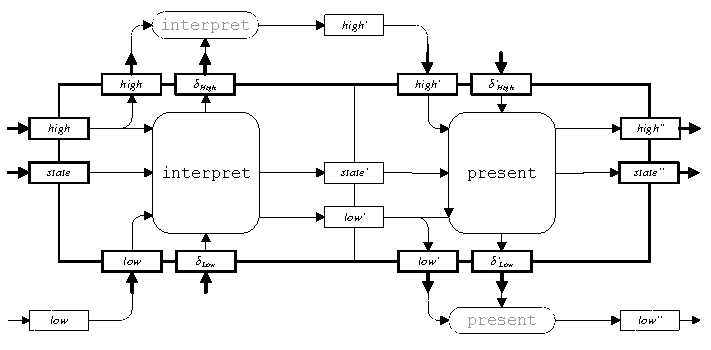
\includegraphics[width=\columnwidth]{images/LayerDataFlow}
\caption{Data flow in a Proxima layer.} \label{proximaDataFlow}
\end{figure}



\bc
The main difference between a Proxima layer and a \p{Simple} layer is that in Proxima, the data levels are part of the horizontal data flow. The vertical data flow consists of edit operations. Furthermore, the first step in a Proxima layer is \p{interpret} instead of \p{present}.

Note that the identifiers represent values, and not type variables. The dotted arrows outside the layer sketch the data flow of the higher and lower levels in the adjacent layers. Besides the lower-level edit operation $\delta_{Low}$, \p{interpret} gets both levels and a $state$ argument (which is explained below). The result of \p{interpret} is the higher level edit operation $\delta_{High}$, and a new $state'$. Moreover, \p{interpret} returns $low'$, which is the result of applying $\delta_{Low}$ to $Low$. The behavior of \p{present} is symmetrical.

The figure also shows how the higher level is updated by \p{interpret} of layer above, before coming back down as $high'$. Similarly, \p{present} of the layer below updates $low'$ to $low''$. 

The $state$ parameter represents the local state for a layer. It should not be confused with extra state, which is part of the level. Local layer state is information that is needed by a layer, but belongs to the layer rather than to one of the adjacent levels. An example is a reference to a font metrics table in the arrangement layer.

At the top of the combined layers, the document and edit operation resulting from interpretation are passed back as arguments to the presentation step. And at the bottom, an edit gesture from the user must be put into the combined layers combination, and an updated rendering is be shown to the user. 
\ec

The data flow in the figure is encoded in the type definition for a Proxima layer. For the edit operations (the $\delta$'s in Figure~\ref{proximaDataFlow}), we use distinct types for edit operations going up (\p{editH} and \p{editL}) and edit operations going down (\p{editH'} and \p{editL'}). The reason for this distinction is that upward edit operations are often of a different nature than the downward ones. The code below is actual Proxima source code:

\begin{small}
\begin{verbatim}
data Layer m state high low editH editL editH' editL' =
       Layer { interpret ::
                 LayerFn m (state, high) (low, editL)
                           (state, low) (high, editH)
             , present ::
                 LayerFn m (state, low) (high, editH')
                           (state, high) (low, editL')
             }
\end{verbatim}
\end{small}

The \p{Layer} definition is part of the \p{Architecture} module, which imports the modules that define \p{interpret} and \p{present} for each layer. The definitions of the layer type as well as \p{lift} and \p{combine} for Proxima are the same as for the simple editor, except for the fact that \p{present} and \p{interpret} are swapped. The Proxima main edit loop is also virtually the same, except that it consists of more layers than the simple editor.


\bc
\bigskip

The architecture combinators enforce a a strict separation between the different layers. In some cases, this . However, in general it leads to a very compositional system in which the data flow is very transparent. The addition of a new layer. Furthermore the strict separation also helped to keep user interface dependent code ... to only a few modules. Hence, adapting the system for a different user interface is not a major operation.

\bl
\o same problem as with type system. Restricting, but enforcess correctness
\o separation, all connections explicit. Very easy to add a new layer. 
\o in contrast to editors in which UI directly updates document.
\el
\ec

\bc
The motivation for using Haskell to describe editor architectures has come from the Proxima project. Proxima is a generic incremental XML editor, which is being developed at Utrecht University. The editor is parameterized with a presentation sheet that specifies how a document is presented. Furthermore, it is parameterized with a computation sheet that specifies derived values, such as chapter numbers, or a table of contents. A user can only see and edit the final presentation of the document. Because the mapping of the document on the presentation is a stepwise process, and hence the interpretation*** from edit commands on the presentation to updates on the document as well, Proxima has a layered architecture.
\ec


\bc
%																
%																
%																
\section{Related work} \label{sect:relatedWork}


The requirements for a DSEL for describing architectures are slightly different from the requirements for more familiar applications of DSELs, such as parsers, pretty printers, etc. The latter are used to write programs that contain many applications of the combinators and that are usually subject to frequent change and frequent use. An architecture description, on the other hand, will typically be a small and rather static entity, because changes to the architecture involve changes to many components of the system. The first association many have with the term ``Architecture Description Language'' is a graphical design environment, in which one can sketch the architecture. Futere work thus incorporates the use of Proxima for bulding such editing environments: the use sees and manipuates a graphical representation, whereas the model is actually a Haskell program. In this research we will build upon work done already in another context: the manipulation of Bayesian networks \cite{schrage05Dazzle}. 
\ec



%																
%																
%																
\section{Conclusions and future work} \label{sect:conclusions}

The combinators presented in this paper make it possible to specify layered editor architectures in a concise and transparent way. With a small number of definitions, a layered architecture can be described, clearly showing the data flow between the layers. The combinators have been heap profiled to ensure that no memory leaks are present, and have been used to implement the Proxima prototype as well as a database web-interface system.

Because the architecture description language is embedded in the implementation language, the architecture of a system forms part of the implementation of the system. We do not need to translate the architecture to an implementation, and hence, the implementation is guaranteed to comply with the architecture and vice versa.

According to Medvidovic and Taylor~\cite{medvidovic00ADLs}, an architecture description language should describe the components of an architecture, the connectors, and the configuration. For the architecture combinators defined in this paper, we can identify these aspects as follows: the layer functions are the components; \p{lift} and \p{combine} are the connectors; and the applications of \p{lift} and \p{combine} determine the configuration.

In the paper we have assumed that once we call a (combined) step function, the information flows through all the layers. In a real editor this might not always be the case; if the user adds some extra white-space this might be recorded in the state at one of the intermediate levels, upon which the presentation process can be resumed. We can also envision a situation where information flows up and down a few times between two adjacent layers, until a situation is reached in which a change has to be propagated to yet another layer. Note that we actually only require that the upper protocol of a lower layer corresponds to the lower protocol of its upper layer; the updating of the document and providing the gesture at the bottom layer are examples of simple single-step protocols. We foresee however that we might use the type system to describe much more complicated protocols. An open question, and a matter of debate, is whether this should be done by exploiting the Haskell type system further, or whether one should move to more expressive type systems such as found in Agda \cite{norell:thesis}. Only experimenting and comparing solutions can give a definitive answer. Another area of research concerns how dynamic aspects of the architecture, such as invariants and constraints on the data, can be described and, if possible, verified.

The combinator language in this paper is tailored to a specific kind of architectures: those of layered editors. Although we use the term editor in a broad sense, also including spreadsheets, e-mail agents, etc., further research should explore the possibilities of using Haskell to describe other kinds of architectures. For us the experiment to model the structure of the system using Haskell has been a successful experience, and we hope that this paper will inspire others to pursue the approach for different classes of architectures.  

\bc
Ik heb geen tijd gehad om dit te bekijken, maar de abstrcat wijst misschien in onze richting
http://portal.acm.org/citation.cfm?id=1035167.1035203&coll=ACM&dl=GUIDE&CFID=33547895&CFTOKEN=34186200
\ec%																									




%\acks


%%%%%%%%%%%%%%%%%%%%%%%%%%%%%%%%%%%%%%%%%%%%%%%%%%%%
%%%%%%%%%%%%%%%%%%%%%%%%%%%%%%%%%%%%%%%%%%%%%%%%%%%%
\bibliographystyle{plainnat}

\bibliography{../proxima}

\end{document}

